\documentclass[12pt]{article}

\title{The VEX Experiments}
\author{Diego Contreras - JGHS Sophomore}
\date{4 February 2021}

\usepackage{hyperref}
\usepackage{biblatex}
\addbibresource{Cites.bib}

\usepackage{graphicx}
\graphicspath{ {./images/} }


\begin{document} % Creates the scope for this document.
\maketitle
\newpage
\tableofcontents
\begin{abstract}
\LaTeX{} is a great typesetting software that builds upon \TeX, a program that allows one to write down mathemathical symbols easily. Anyway, this page is meant to show you that you can create an abtract page in \LaTeX{} very easily by typing \texttt{\textbackslash begin\{abstract\}}.
\end{abstract}
\section{Low-latency Wireless Camera}

I propose two different methods for low-latency, wireless, cheap video transmission: Mobile Device and Raspberry Pi transmission. 

\subsection{Mobile Device Transmission}

Phones are robust computers that are perfect for wireless video transmission due to their decent battery, camera, and wireless capabilities. Without trying to hack the phone, I did an experiment on the following apps for wireless video transmission: \href{https://play.google.com/store/apps/details?id=com.skype.raider&hl=en_US}{Skype}, \href{https://play.google.com/store/apps/details?id=cx.ring&hl=en_US}{Jami}, and \href{https://play.google.com/store/apps/details?id=com.pas.webcam&hl=en_US}{IPWebcam}. Based on speculation and googling, these apps were specifically chosen for their completely different architectures for video transmission, with Skype using a central server to relay peer to peer connections, Jami being completely peer to peer, and IP Webcam streaming video to a local webserver.

To determine which app has the best performance, I ran each app with very similar settings on the same network at 480p on three different Android phones and measured their latencies based on the offset, in milliseconds, there was when the app streamed a clock from my computer back into my computer. Specifically, each app streamed a millisecond-accurate clock from my 60hz display that was accurate to about 17 milliseconds. From there, a built-in screenshot app in my computer was used to capture a picture of the streamed clock and the actual clock and the latency was based off that. Using a python script and \href{https://pypi.org/project/pytesseract/}{pytesseract}, I automated this process for over an hour for each app on each phone. Overall, IP Webcam always had the lowest mean latency for each phone, especially the Stylo 6 at a latency of 164.80 milliseconds, most likely making it the best app on here.

\begin{figure}[h]
\begin{centering}
Phone-App Latency Table\\[0.5cm]

\begin{tabular}{c|c|c|c}
    & Skype Avg. & Jami Avg. & IP Webcam Avg. \\[0.5cm]
    On5 & 365.10 ms & 268.30 ms & 205.10 ms \\[0.5cm]
    Blade Max & 393.03 ms & 313.30 ms & 268.60 ms \\[0.5cm]
    Stylo 6 & 729.70 ms & 301.90 ms & 164.80 ms
\end{tabular} \newline
\end{centering}
\end{figure}

At 480p on a 2.4 ghz network, IP Webcam is the most viable option. With indirect touch, the human eye can perceive latency at around 100 ms \cite{LatencyStudy}, so this method isn't that far off from being noticably instant. Playing around with the settings on a 5 ghz network, I was able to get an average latency of 135.47 ms with a bandwidth of less than 1 Mbps with 352x288 video resolution + 20\% Quality on the Stylo 6, making the camera very fast, usable, and cheap to deploy and use even on a crowded network.

\subsection{Raspberry Pi Transmission}
The only thing as mobile as a phone with the same capabilities at a cheap cost was a Raspberry Pi. Like mobile devices, a Raspberry Pi is a miniature computer that can do all sorts of tasks. The only difference here is that the Raspberry Pi is \textit{full-fledged} computer running on a version of Linux with a much more powerful processor, wifi card, and memory. Using the \href{https://www.raspberrypi.org/products/camera-module-v2/}{Raspberry Pi Camera Module} and a multi-media library called \href{https://gstreamer.freedesktop.org/}{Gstreamer}, I wrote a quick command to stream video from the Raspberry Pi to my computer through a local 5 ghz network. 

\begin{figure}[h]
\begin{centering}

\textit{Command for Raspberry Pi (Sender)}

\texttt{raspivid -n -t 0 -w \{width\} -h \{height\} -qp \{quality\} -fps \{fps\} --flush -b \{bitrate\} -o - | gst-launch-1.0 -e -vvvv fdsrc ! h264parse ! rtph264pay config-interval=1 pt=96 ! udpsink host=\{Linux Machine IP\} port=\{UDP port\}} \\[1cm]

\textit{Command for Linux Machine (Receiver)}

\texttt{gst-launch-1.0 -e -v udpsrc address=\{Linux Machine IP\} port=\{UDP port\} ! application/x-rtp, payload=96 ! rtpjitterbuffer ! rtph264depay ! avdec\_h264 ! autovideosink sync=false}
\end{centering}
\end{figure}

The sender command says this: feed the H.264 video feed of the Raspberry Pi's camera (\texttt{raspivid}) into \texttt{gst-launch-1.0} (gstreamer) via the pipe operator \texttt{|} so that it gets sent to the receiver via a UDP connection. The receiving command simply decodes the data into a window.

\begin{figure}[!htb]
    \centering
    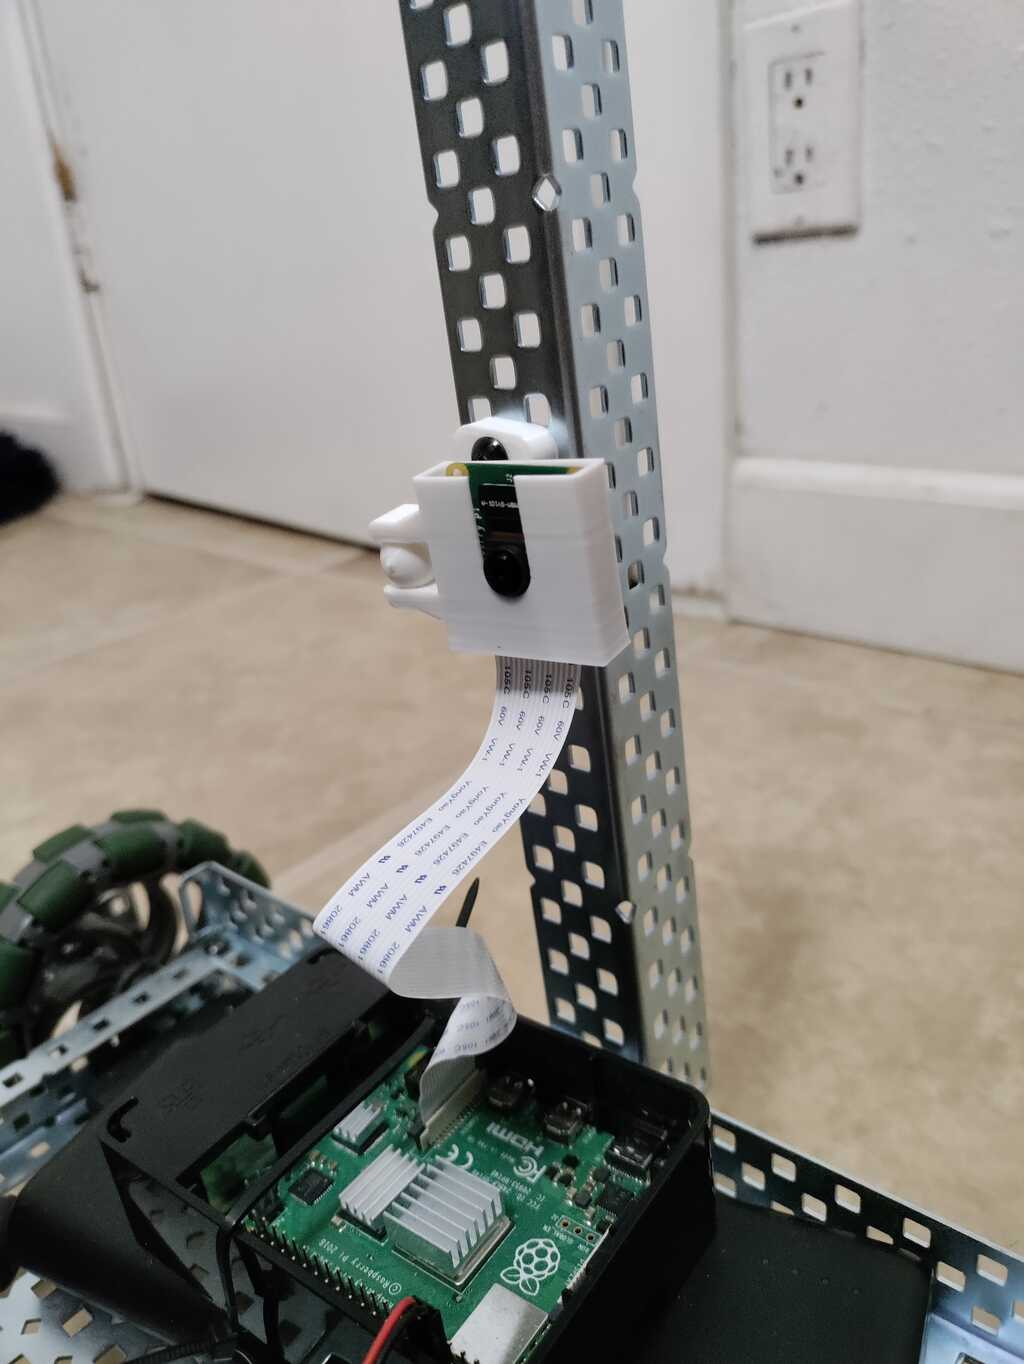
\includegraphics[width=\textwidth,height=6cm,keepaspectratio=true]{IPCamera/3DRaspCustom}
    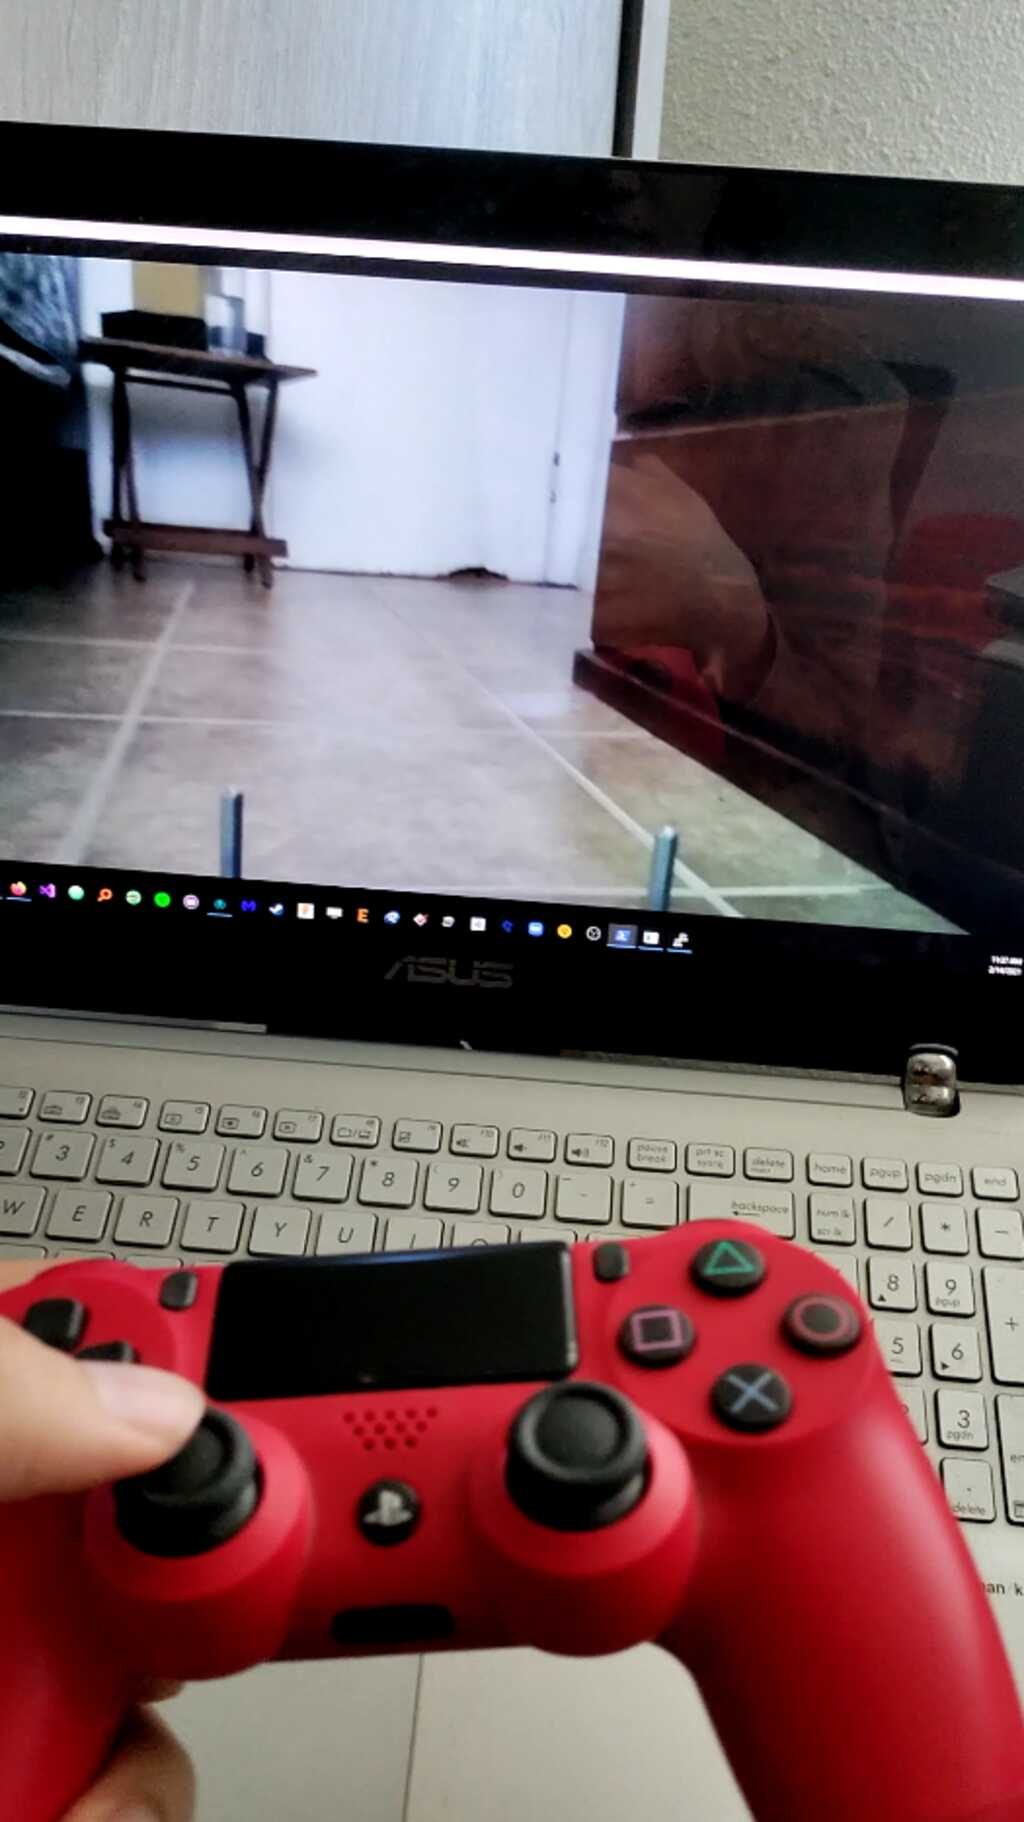
\includegraphics[width=\textwidth,height=6cm,keepaspectratio=true]{IPCamera/RemoteController}
    \caption{
        (Left) Raspberry Pi Camera mounted via a 3D printed part. (Right) Live video feed of the camera.
    }
\end{figure}


Unfortunately, I am too lazy to measure how fast this approach is compared to phones. However, I can say, from experience, that this setup can stream 720p with less than 150 ms of latency at 30 fps; Something unheard of in weak Android phones. Due to this, I would consider using this camera as the main camera, with phone acting as backups / side cameras.



\newpage
\section{Effective Robot Design}
% Arm math
% Differential Drive explains wheel placement
% Better nuts

\newpage
\section{Accurate Encoders}
\label{section:accu_encoders}

\newpage
\section{Odometry} % Differential Drive
% Better encoder placement

\newpage
\section{The Batteries}
% New method of testing batteries

\newpage
\section{3D Printing}

\newpage
\section{Driving}
% Raspberry Pi
% Partner controllers

\newpage
\section{The Club}
% Pizza
% Determine work and deadlines
% How we "hire"
% A bit laxer rules
% Emphasis on learning

\printbibliography


\end{document}
